\documentclass[10pt]{beamer}

  % Math Packages
  \usepackage{amsmath}
  \usepackage{amsthm}
  \usepackage{booktabs}
  \usepackage{mathtools}

  % Graphics Packages
  \usepackage{graphicx}
  \usepackage[export]{adjustbox}

  % Style and util packages
  \usepackage{caption}
  \usepackage{dirtytalk}

  % Bibliography
  \usepackage{hyperref}
  \usepackage{natbib}
  \bibliographystyle{ecta}

  % Theme Settings
  \usetheme{metropolis}
  \usefonttheme{professionalfonts}

  \hypersetup{
    % colorlinks=true,  % false: boxed links; true: colored links
    % linkcolor=red,  % color of internal links (change box color with linkbordercolor)
    citecolor=blue,  % color of links to bibliography
    % urlcolor=red  % color of external links
  }

  % Colors
  \definecolor{myred}{rgb}{1.0, 0.11, 0.0}
  \definecolor{mygreen}{rgb}{0.13, 0.55, 0.13}

\title{Dissertation Defense}
\author{Chase Coleman}
\institute{NYU Stern}
\date[]{\today}

\begin{document}

% Title Slide
\begin{frame}
  \thispagestyle{empty}
  \titlepage
\end{frame}

% --------------------------------------- %
% Introduction
% --------------------------------------- %
\begin{frame} \frametitle{What have I learned?}

  Three Chapters:

  \vspace{0.5cm}

  \begin{enumerate}
    \item Pareto weights as wedges in two-country models (with Dave Backus, Axelle Ferriere,
          and Spencer Lyon)
    \item Global solution methods for macroeconomic models (with Spencer Lyon, Lilia Maliar, and
          Serguei Maliar)
    \item Cost of income-driven repayment for student loans
  \end{enumerate}

\end{frame}

% -------------------------------------------- %
% Pareto weights as wedges in two-country models
% -------------------------------------------- %
\section{Pareto weights as wedges in two-country models}

  \begin{frame} \frametitle{Introduction}

    \textbf{Environment}: Recursive preferences in a typical two country, two (tradeable) goods,
    exchange economy (a la Backus Kehoe Kydland 1994).

    \vspace{0.25cm}

    \textbf{Want}: Understand the stochastic process that governs the relative pareto weights in a
    two country economy with recursive preferences

    \vspace{0.5cm}

    \textbf{What did we learn?}:

    \begin{itemize}
        \item While in one-good models pareto weights are unstable, a risk adjustment associated
        with the addition of a second good implies stability of the stochastic process governing
        pareto weights.
        \item Time-varying pareto weights imply a ``wedge'' in model that can help address various
        puzzles --- One example is the Backus-Smith puzzle
    \end{itemize}

  \end{frame}

% --------------------------------------------------- %
% Global solution algorithms for macroeconomic models
% --------------------------------------------------- %
\section{Global Solution methods for macroeconomic models}

  \begin{frame} \frametitle{Global solutions}

    Global solutions allow more accurate characterizations of model dynamics than perturbation
    methods. Certain models/questions should not use less accurate methods --- For example, models
    of labor search, sovereign default, and certain classes of NK models.

    \vspace{0.25cm}

    \textbf{Want}: Global solution method that can work reasonably well for ``medium-sized'' (8
    state variable model) so these models can be calibrated.

    \vspace{0.25cm}

    \textbf{Solution}: Perturbation of \textit{Epsilon-distinguishable sets} methods. Rather than
    simulate to get grid, use pseudo-random points in hypercube.

    \vspace{0.25cm}

    \textbf{Performance}: See 50x speed up related to EDS and can solve 8-state model in
    about a second.

  \end{frame}


% --------------------------------------------------- %
% Cost of income-driven student loans
% --------------------------------------------------- %
\section{Cost of income-driven student loans}

  \begin{frame} \frametitle{U.S. student loan repayment plans}

    \begin{table}
      {\small
      \hspace*{-0.5cm}\begin{tabular}{lll}
        \toprule
        \textbf{Name} & \textbf{Payment} & \textbf{Forgiveness} \\
        \midrule
        {\color{myred} AMR} & Amortized over 10 years & None \\
        {\color{myred} Graduated} & Fixed schedule which increases over 10 years & None \\
        {\color{mygreen} IBR} & 15\% of disposable income (up to AMR) & 25 years \\
        {\color{mygreen} REPAYE} & 10\% of disposable income & 20 years \\
        {\color{mygreen} Trump Proposal} & 12.5\% of disposable income & 15 years \\
        \bottomrule
      \end{tabular}
      }
    \end{table}

  \end{frame}

  \begin{frame} \frametitle{Hard to determine cost}

     \begin{figure}
       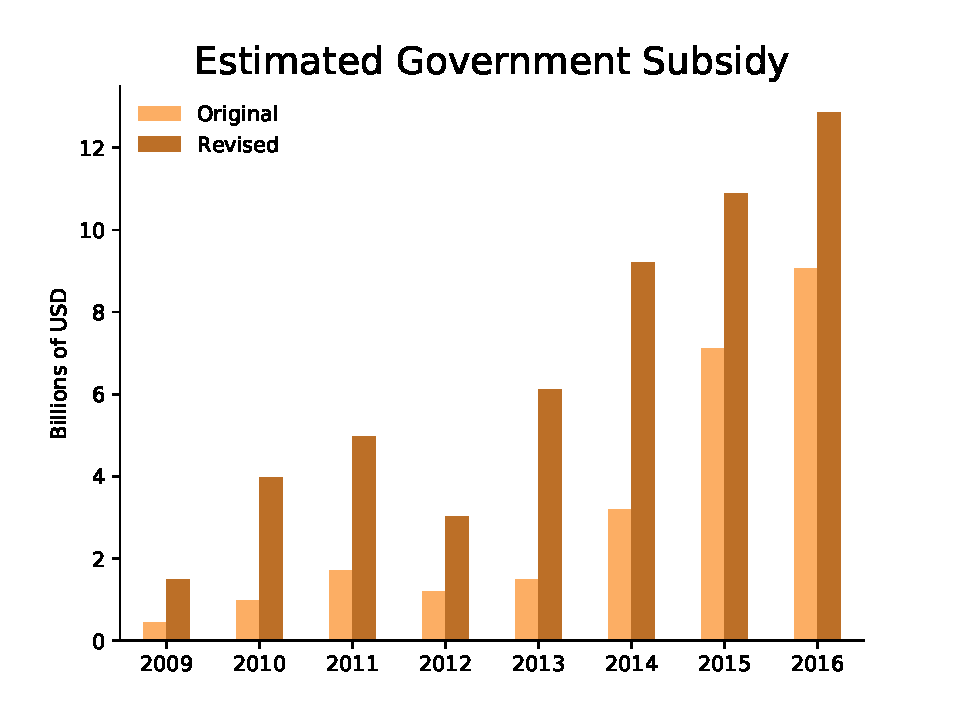
\includegraphics[width=\textwidth]{../ms/images/StudentLoans/GovSubsidy_Original_v_Revised.pdf}
       \caption*{\tiny{GAO analysis of the U.S. Department of Educations' 2011-2017 budget estimates; \cite{GAO-17-22}}}
     \end{figure}

  \end{frame}

  \begin{frame} \frametitle{Hard to determine cost}

    \say{
        \dots there are a number of factors that make forecasting future IDR participation
        inherently difficult\dots it entails behavioral effects that are extremely difficult to
        incorporate and project into the future --- Department of Education response to
        Goverment Accountability Office
    }

  \end{frame}

  \begin{frame} \frametitle{Paper counterfactual}

    In this paper, I run the following counterfactual:

    \vspace{0.25cm}

    Consider two economies

    \begin{enumerate}
      \item All student loans held in AMR repayment plan
      \item All student loans held in IDR repayment plan
    \end{enumerate}

    Will determine how much it costs for the government to support IDR relative to AMR

  \end{frame}

  \begin{frame} \frametitle{Government subsidy}

      \textbf{Key variable of interest}: Subsidy required to keep student loans program solvent
      ($\Delta_{SL}$):

      \vspace{0.5cm}

      $$\Delta_{SL} = \sum_i (d_i - X_i)$$

      \vspace{0.5cm}

      where $d_i$ is debt accumulated by individual $i$ and $X_i$ is the present discounted value
      of the payments they make

  \end{frame}

  \begin{frame} \frametitle{Government subsidy decomposition}

      Decompose $\Delta_{SL}$ by

      \vspace{0.5cm}

      \begin{align*} \label{eq:gov_subsidy}
        \Delta_{SL} &=
            \underbrace{\frac{\sum_i (d_i - X_i)}{\sum_i d_i}}_{\text{subsidy rate}} \times
            \underbrace{\frac{\sum_i d_i}{N_d}}_{\text{average debt}} \times
            \underbrace{\frac{N_d}{N_e}}_{\text{fraction in debt}} \times
            \underbrace{\frac{N_e}{N}}_{\text{enrollment rate}} \times
            N
      \end{align*}

  \end{frame}

  \begin{frame} \frametitle{What we will learn today}

    We find that going from an economy with only AMR to an economy with only IDR results in

    \vspace{0.5cm}

    \begin{itemize}
      \item A 1 pp increase in enrollment rate
      \item 24 pp increase in percent of students with debt
      \item 17\% increase in average student loan size
      \item 50\% increase in subsidy rate
    \end{itemize}

    \vspace{0.5cm}

    These result in a 15\% increase in the cost of running the student loans program

  \end{frame}

  \begin{frame} \frametitle{Model outline: idiosyncratic type}

    All students begin as high school graduates. Draw three idiosyncratic states:

    \begin{itemize}
      \item Ability level ($a$): Unobservable to individuals and will affect the probability with
      which they pass classes in college and their labor earnings.
      \item Type ($j$): Type consists of 4 components $(m, k, q, z)$ --- $m$ is a signal about an
      individual's ability level, $k$ is the initial risk-free holdings, $q$ is the cost of college,
      and $z$ is they yearly parental transfer.
      \item Financial state ($\zeta_1$): Stochastic component of the cost of college and college
      work opportunities.
    \end{itemize}

    Additionally, assume econometrician cannot observe $m$, but rather observes

    $$\text{GPA} = m + \varepsilon_{\text{GPA}}$$

  \end{frame}

  \begin{frame} \frametitle{Model outline}

    \begin{figure}
      \begin{center}
       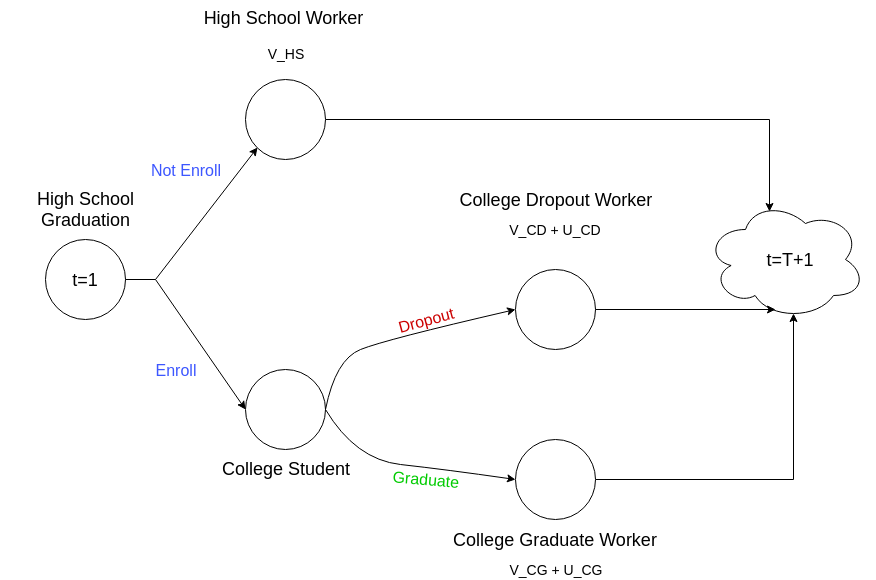
\includegraphics[width=\textwidth]{../ms/images/StudentLoans/LifeCycleChart.png}
      \end{center}
    \end{figure}

  \end{frame}

  \begin{frame} \frametitle{Enrollment effects}

    The probability of enrollment is given by:

    $$\text{prob}(\text{enroll}) = \frac{\exp(V^{S})}{\exp(V^{S}) + \exp(V^{HS})}$$

    \vspace{0.75cm}

    $V^{HS}$ unaffected by changes in repayment plan which means all changes must come through
    changes in $V^{S}$. $V^{S}$ is itself only indirectly affected by changes in $V^{CD}$ and
    $V^{CG}$

  \end{frame}

  \begin{frame} \frametitle{Enrollment effects}

    \begin{figure}
      \begin{center}
       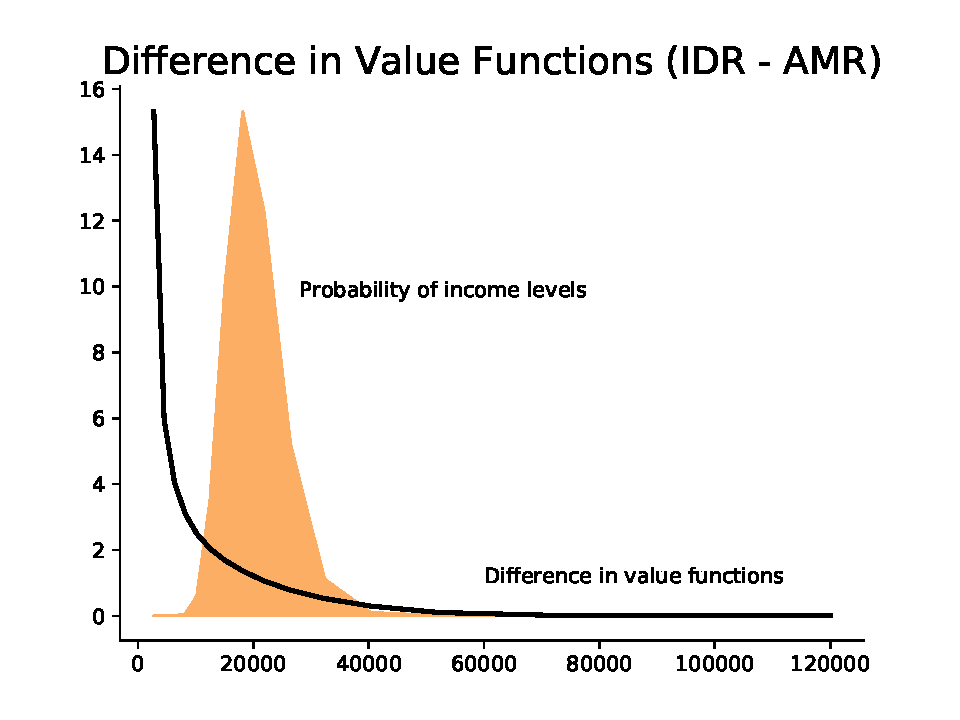
\includegraphics[width=\textwidth]{../ms/images/StudentLoans/vf_vs_income_probs.pdf}
      \end{center}
    \end{figure}

  \end{frame}

  \begin{frame} \frametitle{Debt effects}

    \begin{figure}
      \begin{center}
       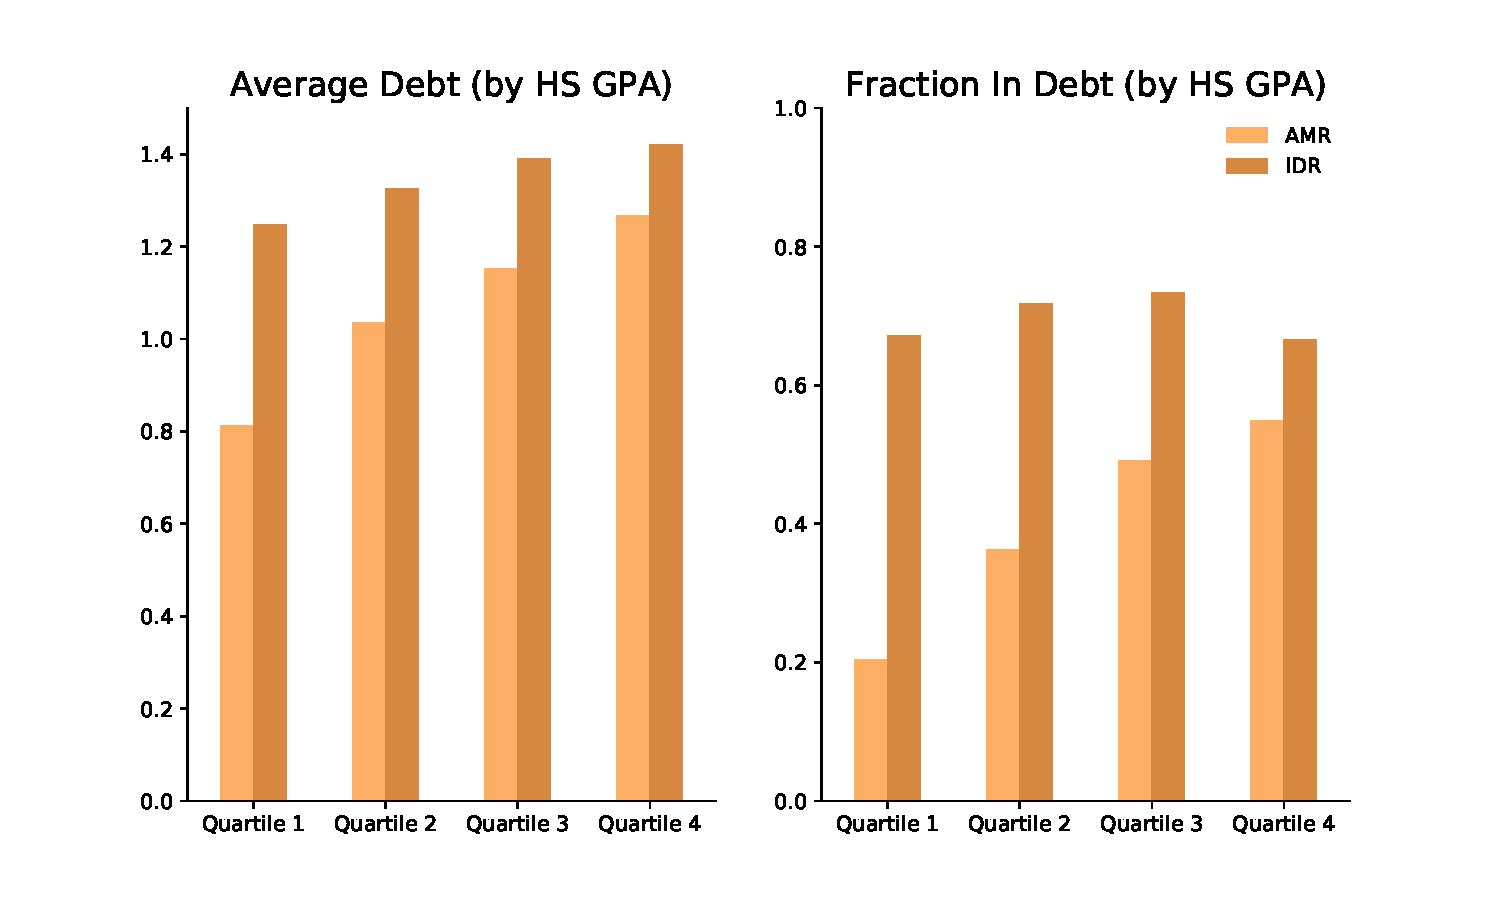
\includegraphics[width=\textwidth]{../ms/images/StudentLoans/DebtByGPA.pdf}
      \end{center}
    \end{figure}

  \end{frame}

  \begin{frame} \frametitle{Debt effects: Thought experiment}

    Imagine that an individual gets an information shock at beginning of the last period of their
    college degree.

    \vspace{0.1cm}

    They find out that they will experience low income for 20 years and, at their current student
    loan level, will experience loan forgiveness. What are implications for student loan
    accumulation this period?

    \vspace{0.1cm}

    If forgiveness, $\frac{\partial V^{CD}}{\partial d_t} = 0$ implies
    $\frac{\partial V^{S}}{\partial d_t} > 0$ for all amounts of debt larger than current student
    loans\dots

    \textbf{Optimal response}: Take out maximum level of student loans.

    \vspace{0.3cm}

    Lowest quartile increases debt accumulation the most because highest probability of forgiveness

  \end{frame}

  \begin{frame} \frametitle{Expected repayment by loan size}

    \begin{figure}
      \begin{center}
       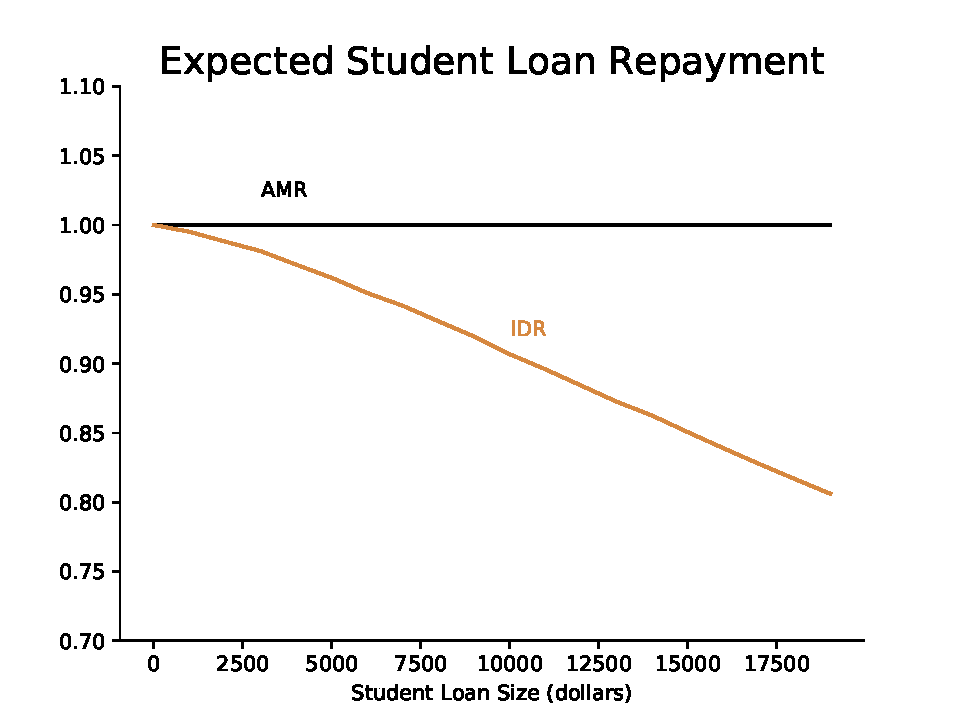
\includegraphics[width=\textwidth]{../ms/images/StudentLoans/expected_repayment.pdf}
      \end{center}
    \end{figure}

  \end{frame}

  \begin{frame} \frametitle{Government subsidy rate by HS GPA quartile}

    \begin{table}[H]
      \begin{tabular}{lll}
        \toprule
        & \textbf{AMR} & \textbf{IDR} \\
        \midrule
        Quartile 1 & -0.13 & 0.11 \\
        Quartile 2 & -0.13 & -0.01 \\
        Quartile 3 & -0.13 & -0.07 \\
        Quartile 4 & -0.13 & -0.11 \\
        \bottomrule
      \end{tabular}
    \end{table}

  \end{frame}

  \begin{frame} \frametitle{Conclusion and next steps}

    IDR is expensive --- More targeted policies to reduce student loan repayment risk may be more
    successful.

    For example, one policy that reduces overall government subsidy in the IDR economy to the level
    from the AMR economy is offering IDR only to those in top 3 GPA quartiles.

    \vspace{0.5cm}

    Occupation choice? Major choice? Higher frequency model to capture more labor market risk?

  \end{frame}

\end{document}
